\section{B-Link-Tree}\label{section:b-link-tree}

Previous approaches include locking a subtree of highest affected node \cite{samadi1976b}, which, albeit straightforward, reduced concurrency. To alleviate the bottleneck without risking inconsistency, \textit{B-Link-Tree} relaxes the definition of B$^+$Trees. As explained by Graefe \cite{goetz-tech}:

\begin{definition}
  B-Link-Tree is a B$^+$Tree with following properties:
  \begin{enumerate}
    \item Each node $x$ has additional attributes:
          \begin{itemize}
            \item $x.\mathit{sibling}$, a pointer to a right sibling node at the same level,
            \item $x.highkey$, the upper bound of all keys found in the subtree rooted by $x$ (every key found in $x$ is less then $x.highkey$).
          \end{itemize}
    \item Does not require locks nor latches for reading.
  \end{enumerate}
\end{definition}

\begin{figure}
  \centering
  \begin{figure}[H]
  \centering
  \begin{tikzpicture}[
    bnode/.style = {
        draw,
        rectangle split,
        rectangle split horizontal,
        rectangle split ignore empty parts,
        anchor=north
      },
    bchild/.style = { -> },
    bsibling/.style = { ->, red },
    bvalue/.style = { -{Circle[open]}, blue }
    ]

    % Level 0
    \node[bnode](y0) {
      \nodepart{one} $4$ \nodepart{two} $7$
    };

    % Level 1
    \draw[bchild](y0.south west) -- +(-4,-1) node[bnode](y1x0){
        \nodepart{one} $1$
      };

    \draw[bchild](y0.one split south) -- +(0,-1) node[bnode](y1x1){
        \nodepart{one} $1$ \nodepart{two} $2$
      };

    \draw[bchild](y0.south east) -- +(4,-1) node[bnode](y1x2){
        \nodepart{one} $1$
      };

    \draw[bsibling](y1x0.east) -- (y1x1.west);
    \draw[bsibling](y1x1.east) -- (y1x2.west);

    % Level 2
    \draw[bchild](y1x0.south west) -- +(-0.5,-1) node[bnode](y2x0){
        \nodepart{one} $1$
      };
    \draw[bvalue](y2x0.one south) -- +(0,-0.5);

    \draw[bchild](y1x0.south east) -- +(0.5,-1) node[bnode](y2x1){
        \nodepart{one} $1$ \nodepart{two} $2$
      };
    \draw[bvalue](y2x1.one south) -- +(0,-0.5);
    \draw[bvalue](y2x1.two south) -- +(0,-0.5);

    % ------
    \draw[bchild](y1x1.south west) -- +(-1.5,-1) node[bnode](y2x2){
        \nodepart{one} $1$
      };
    \draw[bvalue](y2x2.one south) -- +(0,-0.5);

    \draw[bchild](y1x1.one split south) -- +(0,-1) node[bnode](y2x3){
        \nodepart{one} $1$ \nodepart{two} $2$
      };
    \draw[bvalue](y2x3.one south) -- +(0,-0.5);
    \draw[bvalue](y2x3.two south) -- +(0,-0.5);

    \draw[bchild](y1x1.south east) -- +(1.5,-1) node[bnode](y2x4){
        \nodepart{one} $1$ \nodepart{two} $2$
      };
    \draw[bvalue](y2x4.one south) -- +(0,-0.5);
    \draw[bvalue](y2x4.two south) -- +(0,-0.5);

    % ------
    \draw[bchild](y1x2.south west) -- +(-0.5,-1) node[bnode](y2x5){
        \nodepart{one} $1$ \nodepart{two} $2$
      };
    \draw[bvalue](y2x5.one south) -- +(0,-0.5);
    \draw[bvalue](y2x5.two south) -- +(0,-0.5);

    \draw[bchild](y1x2.south east) -- +(0.5,-1) node[bnode](y2x6){
        \nodepart{one} $1$
      };
    \draw[bvalue](y2x6.one south) -- +(0,-0.5);

    \draw[bsibling](y2x0.east) -- (y2x1.west);
    \draw[bsibling](y2x1.east) -- (y2x2.west);
    \draw[bsibling](y2x2.east) -- (y2x3.west);
    \draw[bsibling](y2x3.east) -- (y2x4.west);
    \draw[bsibling](y2x4.east) -- (y2x5.west);
    \draw[bsibling](y2x5.east) -- (y2x6.west);

  \end{tikzpicture}
  \caption{B-Link-Tree with $\mathit{Order} = 3$}
\end{figure}

  \caption{B-Link-Tree with $\mathit{Order} = 3$.}
\end{figure}

Splitting during node insertion is divided into two independent steps: splitting a node and inserting the split node with its new separator key to the parent node.

\begin{figure}[H]
  \centering
  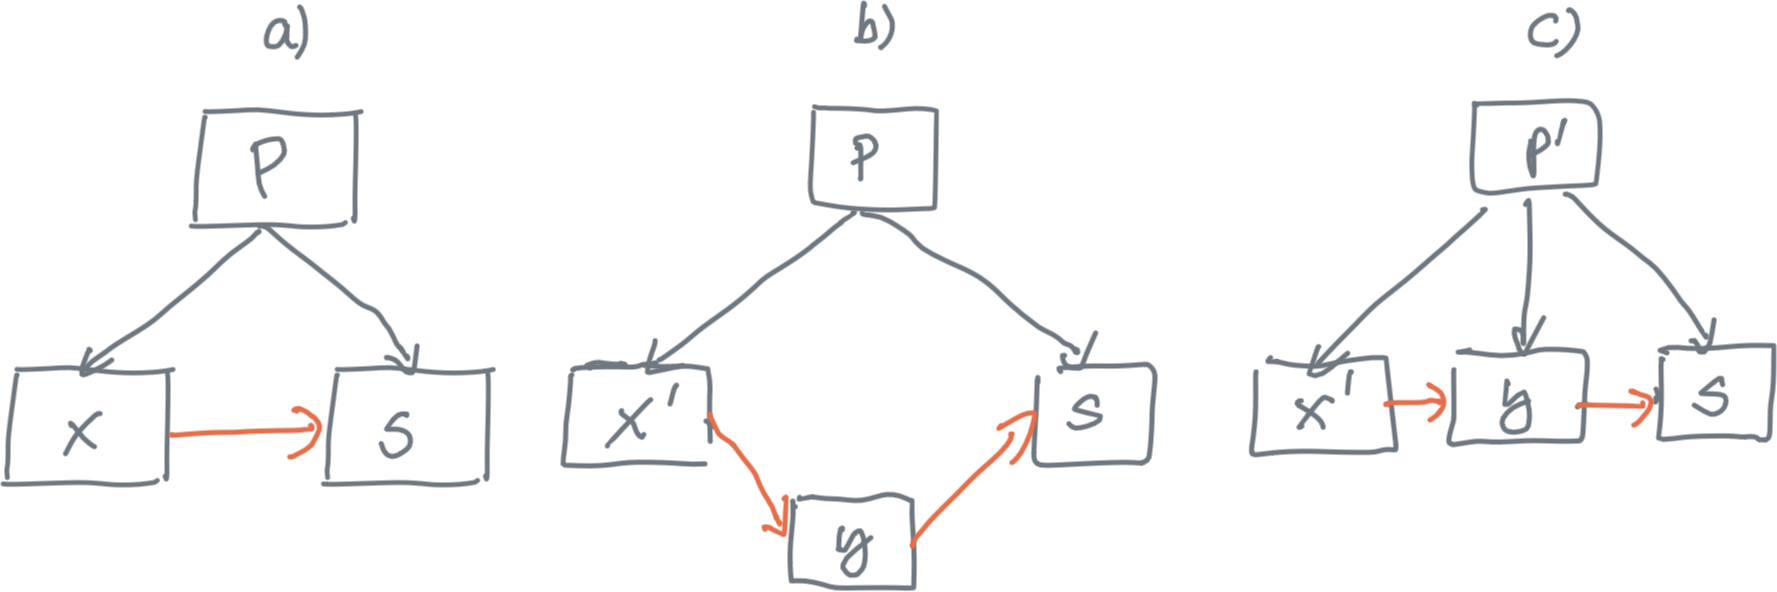
\includegraphics[width=0.8\textwidth ]{components/figure/b-link-insert}
  \caption{States of the tree during splitting while inserting a new key.}
  \label{figure:b-link-insert}
\end{figure}

Assuming node $x$ is a full node, which needs to be split, shown in step (a) in \cref{figure:b-link-insert}. When splitting the node $x$, a new right sibling node $y$ is created, as seen in step (b). The node $y$ inherits the high key from the split node $x$, whereas the $x$ node is updated (marked as $x^\prime$) with a new $x.highkey = y.key_0$. Thus, an internal node does exist without a parent in between the operations.

$x^\prime.highkey$ is used to be able to traverse the newly split node and its subtree, even when the split operation is not complete. \todo{refactor this sentence to better clarify the usage of sibling nodes}

As the final step of node splitting, both the separator key and the pointer to the newly split node $y$ are inserted in the parent node $p$, seen in step (c). Similar to the insertion in B-Tree, a split operation might trigger additional splitting in higher levels.

Tree traversal is modified to honor $x.highkey$ by returning the node at $x.\mathit{sibling}$ when the target key $k$ is larger or equal than $x.highkey$.

\subsection{Proof of correctness}

To prove the correctness of each operation performed on the B-link-tree, the following theorems need to be proven: \todo{add proof from yehman}

\begin{itemize}
  \item \textit{Deadlock freedom} --- threads performing operations on the B-link-tree cannot produce a deadlock,
  \item \textit{Correct tree modifications} --- the tree must appear as a valid tree for all nodes at any time,
  \item \textit{Correct interactions} --- concurrent operations do not interfere with one another.
\end{itemize}

\begin{theorem}
  \textit{Deadlock freedom}: threads performing operations on the B-link-tree cannot produce a deadlock.
\end{theorem}

\begin{proof}
  By imposing a total ordering of nodes, cycles are eliminated from the system. Thus the system is deadlock-free.

  To prove a total ordering of nodes, the following ordering $a < b$, where $a$ and $b$ are nodes of the tree, is considered:

  \begin{enumerate}
    \item If $a$ and $b$ are not on the same distance from the root node, then $a < b$ if and only if the path from the root node to node $a$ is shorter than the path from the root node to node $b$ (bottom-up condition),
    \item if $a$ and $b$ are on the same level, then $a < b$ if and only if node $b$ is reachable from node $a$ by following a chain of one or more $sibling$ pointers (left-to-right condition).
  \end{enumerate}

  It can be shown that during insertion operation the total ordering of nodes is preserved. If $a < b$ at time $t_0$ at the start of insertion, then $a < b$ is preserved for $\forall t, t > t_0$, as a node $x$ during split operation will create a node $x^\prime$ and $x^{\prime\prime}$, where $x^\prime < x^{\prime\prime}$ and:

  $$\forall y, y < x \Leftrightarrow y < x^\prime$$
  $$\forall y, x < y \Leftrightarrow x^{\prime\prime} < y$$

  Therefore, insertion will not break the total ordering of nodes.

  Latches for the nodes are acquired by following the ordering; thus, once a latch is acquired for a node, no other latch will be acquired on any node below it, nor on any node on the same level.
\end{proof}

\begin{theorem}\label{theorem:b-link-tree:modifications}
  \textit{Correct tree modifications}: the tree must appear as a valid tree for all nodes at any time.
\end{theorem}

\begin{proof}
  The tree must appear as a valid tree for all threads at any time except for the modifying thread. Assuming writing is done by invoking $\mathit{writeNode}$ function, which will write to the storage atomically.

  The insertion operation, assuming performed on a node $x$ of the tree, will therefore write only in these circumstances:

  \begin{enumerate}
    \item $\mathit{writeNode}(x)$ --- if node $x$ is not considered full and is safe for rewriting,
    \item $\mathit{writeNode}(x^{\prime\prime})$ --- writing a newly allocated node $x^\prime$, which was created in the process of splitting node $x$,
    \item $\mathit{writeNode}(x^{\prime})$ --- rewriting the node $x$ as part of the splitting process, $x.\mathit{sibling}$ is set to point at node $x^\prime$.
  \end{enumerate}

  Even though $\mathit{writeNode}(x^{\prime\prime})$ and subsequent $\mathit{writeNode}(x^\prime)$ operation are done in two writes, it can be shown, that these operations are equivalent to a single change in tree structure:

  \begin{itemize}
    \item When $\mathit{writeNode}(x^{\prime\prime})$ is executed, no other node has a pointer at $x^{\prime\prime}$. Therefore this operation will not modify the tree structure,
    \item when $\mathit{writeNode}(x^\prime)$ is subsequently executed, the $x^\prime.\mathit{sibling}$ is set to point to $x^{\prime\prime}$. This operation therefore does both modify the node $x$ and introduce newly allocated node $x^\prime$ to the tree in a single operation.
  \end{itemize}
\end{proof}

\begin{theorem}
  \textit{Correct interactions}: concurrent operations do not interfere with one another.
\end{theorem}

\begin{proof}
  Assume $t_i$ is the time when the insertion process $I$ writes node $x$ to storage, and $t_r$ is the time when another operation $P$ reads the same node $x$. All of the operations are considered atomic, thus $t_r \neq t_i$.

  First, the case of $t_r > t_i$ is considered: an operation $P$ is reading a node $x$ after the insertion is done. Any changes that the insertion process $I$ does will preserve the correct tree structure, as proven in \cref{theorem:b-link-tree:modifications}.

  In the case of $t_r < t_i$, where insertion $I$ happens after operation $P$ does a read, the proof is broken into three possible scenarios, which the insertion might perform:

  \begin{enumerate}
    \item Simple insertion of a key-pointer pair into node $x$ without splitting,
    \item splitting of node $x$, where the inserted key is placed in the left node $x^\prime$, same as the node, which has been split ($x^\prime = x$),
    \item splitting of node $x$, where the inserted key is placed in the right node $x^{\prime\prime}$, the newly allocated node.
  \end{enumerate}

  In the first scenario, $I$ performs the insertion in node $x$ without additional splitting. If it is inserting into a leaf node ($x.\mathit{leaf} = \mathit{true}$), no other pointers are inserted by the process $I$, and the operation $P$ behaves as if the read happened before insertion.

  If the insertion happens on an internal node ($x.\mathit{leaf} = \mathit{false}$), a key-pointer pair created by splitting a lower-level node $z^{\prime\prime}$ is inserted into the node $x$. This scenario is the only one where a key-pointer pair could propagate upwards to node $x$. The operation $P$ will be able to utilize the link pointers $z.\mathit{sibling}$ to reach both the original node and the newly split node.

  In the second and third scenarios, the process $I$ has split the node $x$ into two nodes $x^\prime$ and $x^{\prime\prime}$. If the process happens on a leaf node, $P$ will continue as if no insertion has occurred. Similar to the first scenario, the only possible scenario where the process $I$ needs to split is when a child node $z$ went through a split and a new separator key and a pointer to $z^{\prime\prime}$.

  Both the insertion and search in the node $z^{\prime\prime}$ below node $x$ will be correct thanks to \cref{theorem:b-link-tree:modifications}. It only remains to prove the correctness of split operation on node $x$.

  Assume $z^{\prime\prime}$ is the node, which has been created by splitting a node below $x$ and $z^\prime$ the node on the left of node $z^{\prime\prime}$ ($z^\prime.\mathit{sibling} = z$). If the search would not follow the pointer of $z$, the operation $P$ will proceed as usual because the nodes $x^\prime$ and $x^{\prime\prime}$ contain the same set of pointers as node $x$ with the addition of the pointer to $z^{\prime\prime}$. Otherwise, if the search would follow the pointer to $z^{\prime\prime}$, had the process $P$ read the node $x$ after the split, the operation $P$ will proceed instead to $z^\prime$ instead. The operation $P$ is then able to reach node $z^{\prime\prime}$ by using the sibling pointer of node $z^\prime$.

  If the process $P$ is another insertion process, it is either searching for the correct node, backtracking upwards, or attempting to insert into node $x$. In the case of searching, the proof is the same as if the process $P$ was a search operation.

  In the case of backtracking, the node $n$ might have been split multiple times since the last read when traversing downwards in the search operation. In this scenario, the insertion process will find the proper target node for insertion using link pointers, as the order between nodes is preserved, and the newly split nodes of node $n$ will be found on the right side of node $n$.

  Finally, the process $P$ can attempt to insert a key (or a key-pointer pair) into node $n$. In this scenario, only one process can hold a latch for the node $n$. After the latch has been acquired by one of the insertion processes, the other will attempt to read the node $n$ afterward. As the read occurs after write, \cref{theorem:b-link-tree:modifications} proves this interaction to be correct.

\end{proof}

